\begin{figure*}[t]
\centering
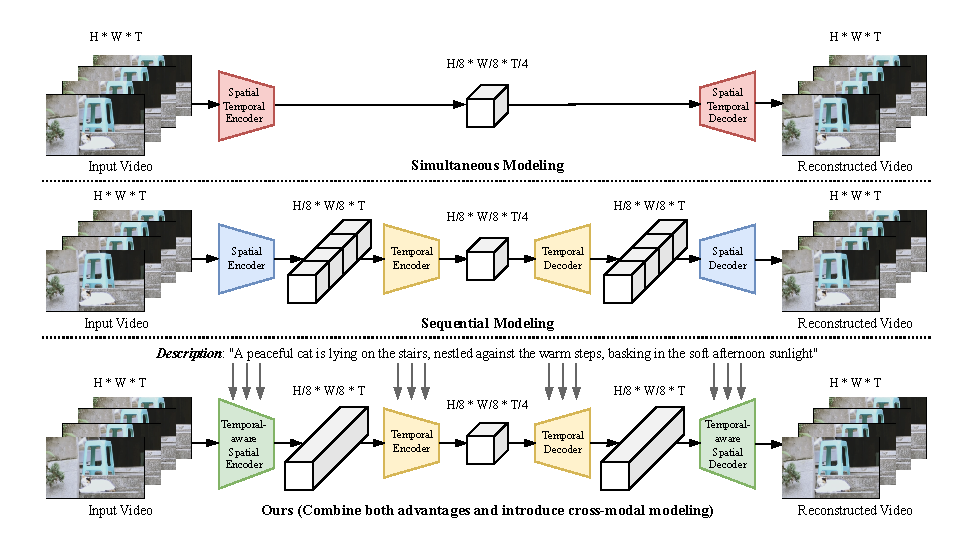
\includegraphics[width=1.0\textwidth]{images/vae_overall3.pdf}
\caption{Comparison of our optimal spatiotemporal modeling and the two other options. Simultaneous modeling is achieved by inflating pre-trained 2D spatial VAE to 3D VAE. Sequential modeling indicates first compressing the spatial dimension with a spatial encoder and then compressing the temporal information with a temporal encoder. 
We identify the issues of these two options and propose to combine both advantages and achieve a much better video reconstruction quality. 
Our VAE also benefits from cross-modality, i.e., text information. 
}
\label{fig:framework}
\vspace{-3mm}
\end{figure*}






\section{Method}


\subsection{Overview}
The video autoencoding problem can be defined as follows. Let $\mathbf{X} \in \mathbb{R}^{C \times T \times H \times W}$ represent a video or image tensor, where $C$, $T$, $H$, and $W$ denote the number of channels, frame(s), height, and width, respectively. We want to train an encoder $\mathcal{E}$ that compresses the input tensor $\mathbf{X}$ into a compact latent representation $\mathbf{Z} \in \mathbb{R}^{C' \times T' \times H' \times W'}$.
%
The learned compact latent $\mathbf{Z}$ can be further reconstructed back to RGB space with decoder $\mathcal{D}$:

\begin{equation}
  \mathbf{Z} = \mathcal{E}({\mathbf{X}}), \hat{\mathbf{X}} = \mathcal{D}(\mathbf{Z}). 
\end{equation}


Our goal is to design and learn such an autoencoder that can reduce the spatial and temporal dimension of video data in latent space and reconstruct the video with highly spatial and temporal fidelity, especially for large-motion scenarios.  


We first examine two inherited video VAE designs from the pre-trained Stable Diffusion model. We then combine the best of two designs and propose our spatiotemporal modeling that can reconstruct high-dynamic contents with fine details. 
We then investigate the text-conditioned video autoencoding and propose an effective text-guided video VAE architecture. 
Moreover, we propose a joint image and video compression training method, that enables text-aided joint image and video autoencoding. Our method does not rely on causal convolution as adopted by prior works. Finally, we carefully study the effects of different loss functions on the reconstruction performance and present the state-of-the-art video VAE architecture. 


\subsection{Optimal Spatiotemporal Modeling}
Designing a video VAE that is inherited from a pre-trained 2D spatial VAE is a good practice to leverage the spatial compression prior. There are typically two options to inflate a 2D spatial VAE to its 3D video counterpart. 

\paragraph{Option 1: Simultaneous Spatiotemporal Compression} One common way to inherit the weight from pre-trained 2D VAE is to inflate the 2D spatial blocks to 3D temporal blocks and simultaneously do the spatial and temporal compression. We first examine this design. Specifically, we replace the 2D convolution in SD VAE with 3D convolution of kernel size (1,3,3), whose weights are initialized from the 2D convolution. Then we add an additional temporal convolution layer with kernel size (3,3,3) to learn spatiotemporal patterns. In this middle block of the inflated VAE, we inflate the 2D attention to 3D attention and we also include a temporal attention to capture both the spatial and temporal information. We keep other components unchanged to maximumly leverage the learned prior of SD VAE. 

\paragraph{Option 2: Sequential Spatiotemporal Compression}
Another reasonable way to cooperate the SD VAE to video VAE is to keep the SD VAE unchanged: first utilize the SD VAE to compress the input video frame-by-frame, and then learn a temporal autoencoding process to further compress the temporal redundancy, as shown in Fig.~\ref{fig:framework}. Specifically, we adopt a lightweight temporal autoencoder for temporal compression. The encoder consists of one convolutional layer to process the input, and two or three 3D ResNet blocks with convolutional downsampling layers to compress the temporal redundancy. Notably, we design the decoder to be asymmetric as the encoder, i.e., there will be two 3D ResNet blocks following each upsampling layer in the decoder. Through this asymmetric design, our decoder can potentially gain some hallucination ability beyond the reconstruction. 

Surprisingly, we find this sequential spatiotemporal design can better compress and recover the dynamic of the input video than option 1, but is not good at recovering spatial details, which is proved by consistent improvement under large-motion video autoencoding as shown in Fig.~\ref{fig:modeling}. 
% . We visualize the results in Fig.~\ref{fig:modeling}. 

\paragraph{Our Solution} We find simultaneous spatiotemporal compression leads to better detail-recovering capability, and the sequential spatiotemporal compression will exceed at motion-recovering ability. Thus, we propose to combine the best of two worlds, and introduce the two-stage spatiotemporal modeling for video VAE. As the first stage, we inflate the 2D convolution to 3D convolution with kernel size (1,3,3), and similarly to option 1, we add additional temporal convolution layers through 3D convolution. We denote our first-stage model as a temporal-aware spatial autoencoder. Different from option 1, we only compress the spatial information and do not compress the temporal information at the first stage, but introduce another temporal encoder to further encode the temporal dimensions, which serves as the second stage compression. We follow the same design of option 2 for our temporal encoder and decoder. After that, we decode the reconstructed latent of the second stage to the RGB space, with the inflated 3D decoder. We jointly train the inflated 3D VAE and the temporal autoencoder. The main idea is illustrated in Fig.~\ref{fig:framework} and Fig.~\ref{fig:2+1D}. 

\paragraph{Formulation}
Recall \( \mathbf{X} \in \mathbb{R}^{C \times T \times H \times W} \) represent a video, where \( C \), \( T \), \( H \), and \( W \) denote the number of channels, frames, height, and width, respectively. The \( i \)-th frame of the video is denoted as \( \mathbf{x}_i \in \mathbb{R}^{C \times H \times W} \). The temporal-aware spatial encoder encodes \( \mathbf{X} \) into a latent representation \( \mathbf{Z}_1 \in \mathbb{R}^{c \times T \times h \times w} \), where \( c \) is the number of latent channels, and \( h = \frac{H}{8} \), \( w = \frac{W}{8} \), as formulated by:

\begin{equation}
    \mathbf{Z}_1 = \mathcal{E}_1(\mathbf{X}).
\end{equation}

Next, the temporal autoencoder encodes \( \mathbf{Z}_1 \) into \( \mathbf{Z}_2 \in \mathbb{R}^{c' \times t \times h \times w} \), where \( c' \) is the number of latent channels for \( \mathbf{Z}_2 \) and \( t = \frac{T}{4} \), as given by:

\begin{equation}
    \mathbf{Z}_2 = \mathcal{E}_2(\mathbf{Z}_1).
\end{equation}

Reconstruction is achieved by decoding \( \mathbf{Z}_2 \) back into the original video space, \( \hat{\mathbf{X}} \in \mathbb{R}^{C \times T \times H \times W} \), through the following inverse process:

\begin{equation}
    \hat{\mathbf{X}} = \mathcal{D}_1(\mathcal{D}_2(\mathbf{Z}_2)) = \mathcal{D}_1(\mathbf{Z}_1).
\end{equation}


\begin{figure}[t]
\centering
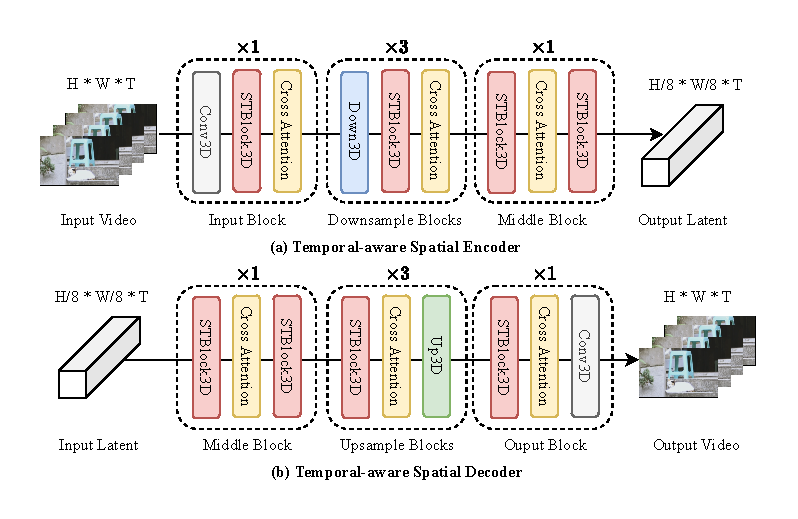
\includegraphics[width=0.5\textwidth]{images/2+1D.pdf}
\caption{The architecture of our temporal-aware spatial autoencoder. We expand the 2D convolution of SD VAE~\cite{rombach2022high} to 3D convolution and append one additional 3D convolution as temporal convolution after the expanded 3D convolution, which forms the STBlock3D. We also inject the cross-attention layers for cross-modal learning with textual conditions. }
\label{fig:2+1D}
\vspace{-3mm}
\end{figure}


\subsection{Cross-modal Modeling}
Since textual information is a native component for text-to-video generation datasets, we examine if the textual information can improve the autoencoding process of the model. To achieve that, we split the feature maps into patches as tokens after each ResNet block in the encoder and decoder, and compute the cross attention by taking visual tokens as query (Q) and value (V), the text embeddings as key (K). 

We try to keep the patch size trackable for each layer. Specifically, we use patch size to 8$\times$8, 4$\times$4, 2$\times$2, and 1$\times$1 for each layer in the temporal-aware spatial autoencoder respectively. We directly use each pixel as one patch in the temporal autoencoder.  We adopt LayerNorm as the normalization function. We use Flan-T5~\cite{t5} as the text embedder. 
A projection convolution is applied to the result, which is then added to the input via a residual connection. 



\subsection{Joint Image and Video Compression}
% \subsection{Cross-modal Modeling}
In contrast to existing architectures such as MagVitV2~\cite{yu2023language}, OD-VAE~\cite{chen2024odvaeomnidimensionalvideocompressor}, and OPS-VAE~\cite{opensora}, which use Causalconv3D layers, we rely primarily on standard Conv3D layer. 


A notable feature of our architecture is the ability to mask out the temporal autoencoder, allowing the first-stage model to operate as a standalone image compressor. 
During training, our model is flexible to take both image and video as input: when the current batch is composed of images, we will disable the temporal convolution and temporal attention layers, as well as the temporal autoencoder. We train our model on both the image dataset and video dataset to let the model learn the image and video compression ability simultaneously. Besides, training on more high-quality images can also help improve the video autoencoding performance. We quantitatively evaluate the performance of our joint image and video compression in Table~\ref{tab:main}. 




\begin{figure*}[t]
\centering
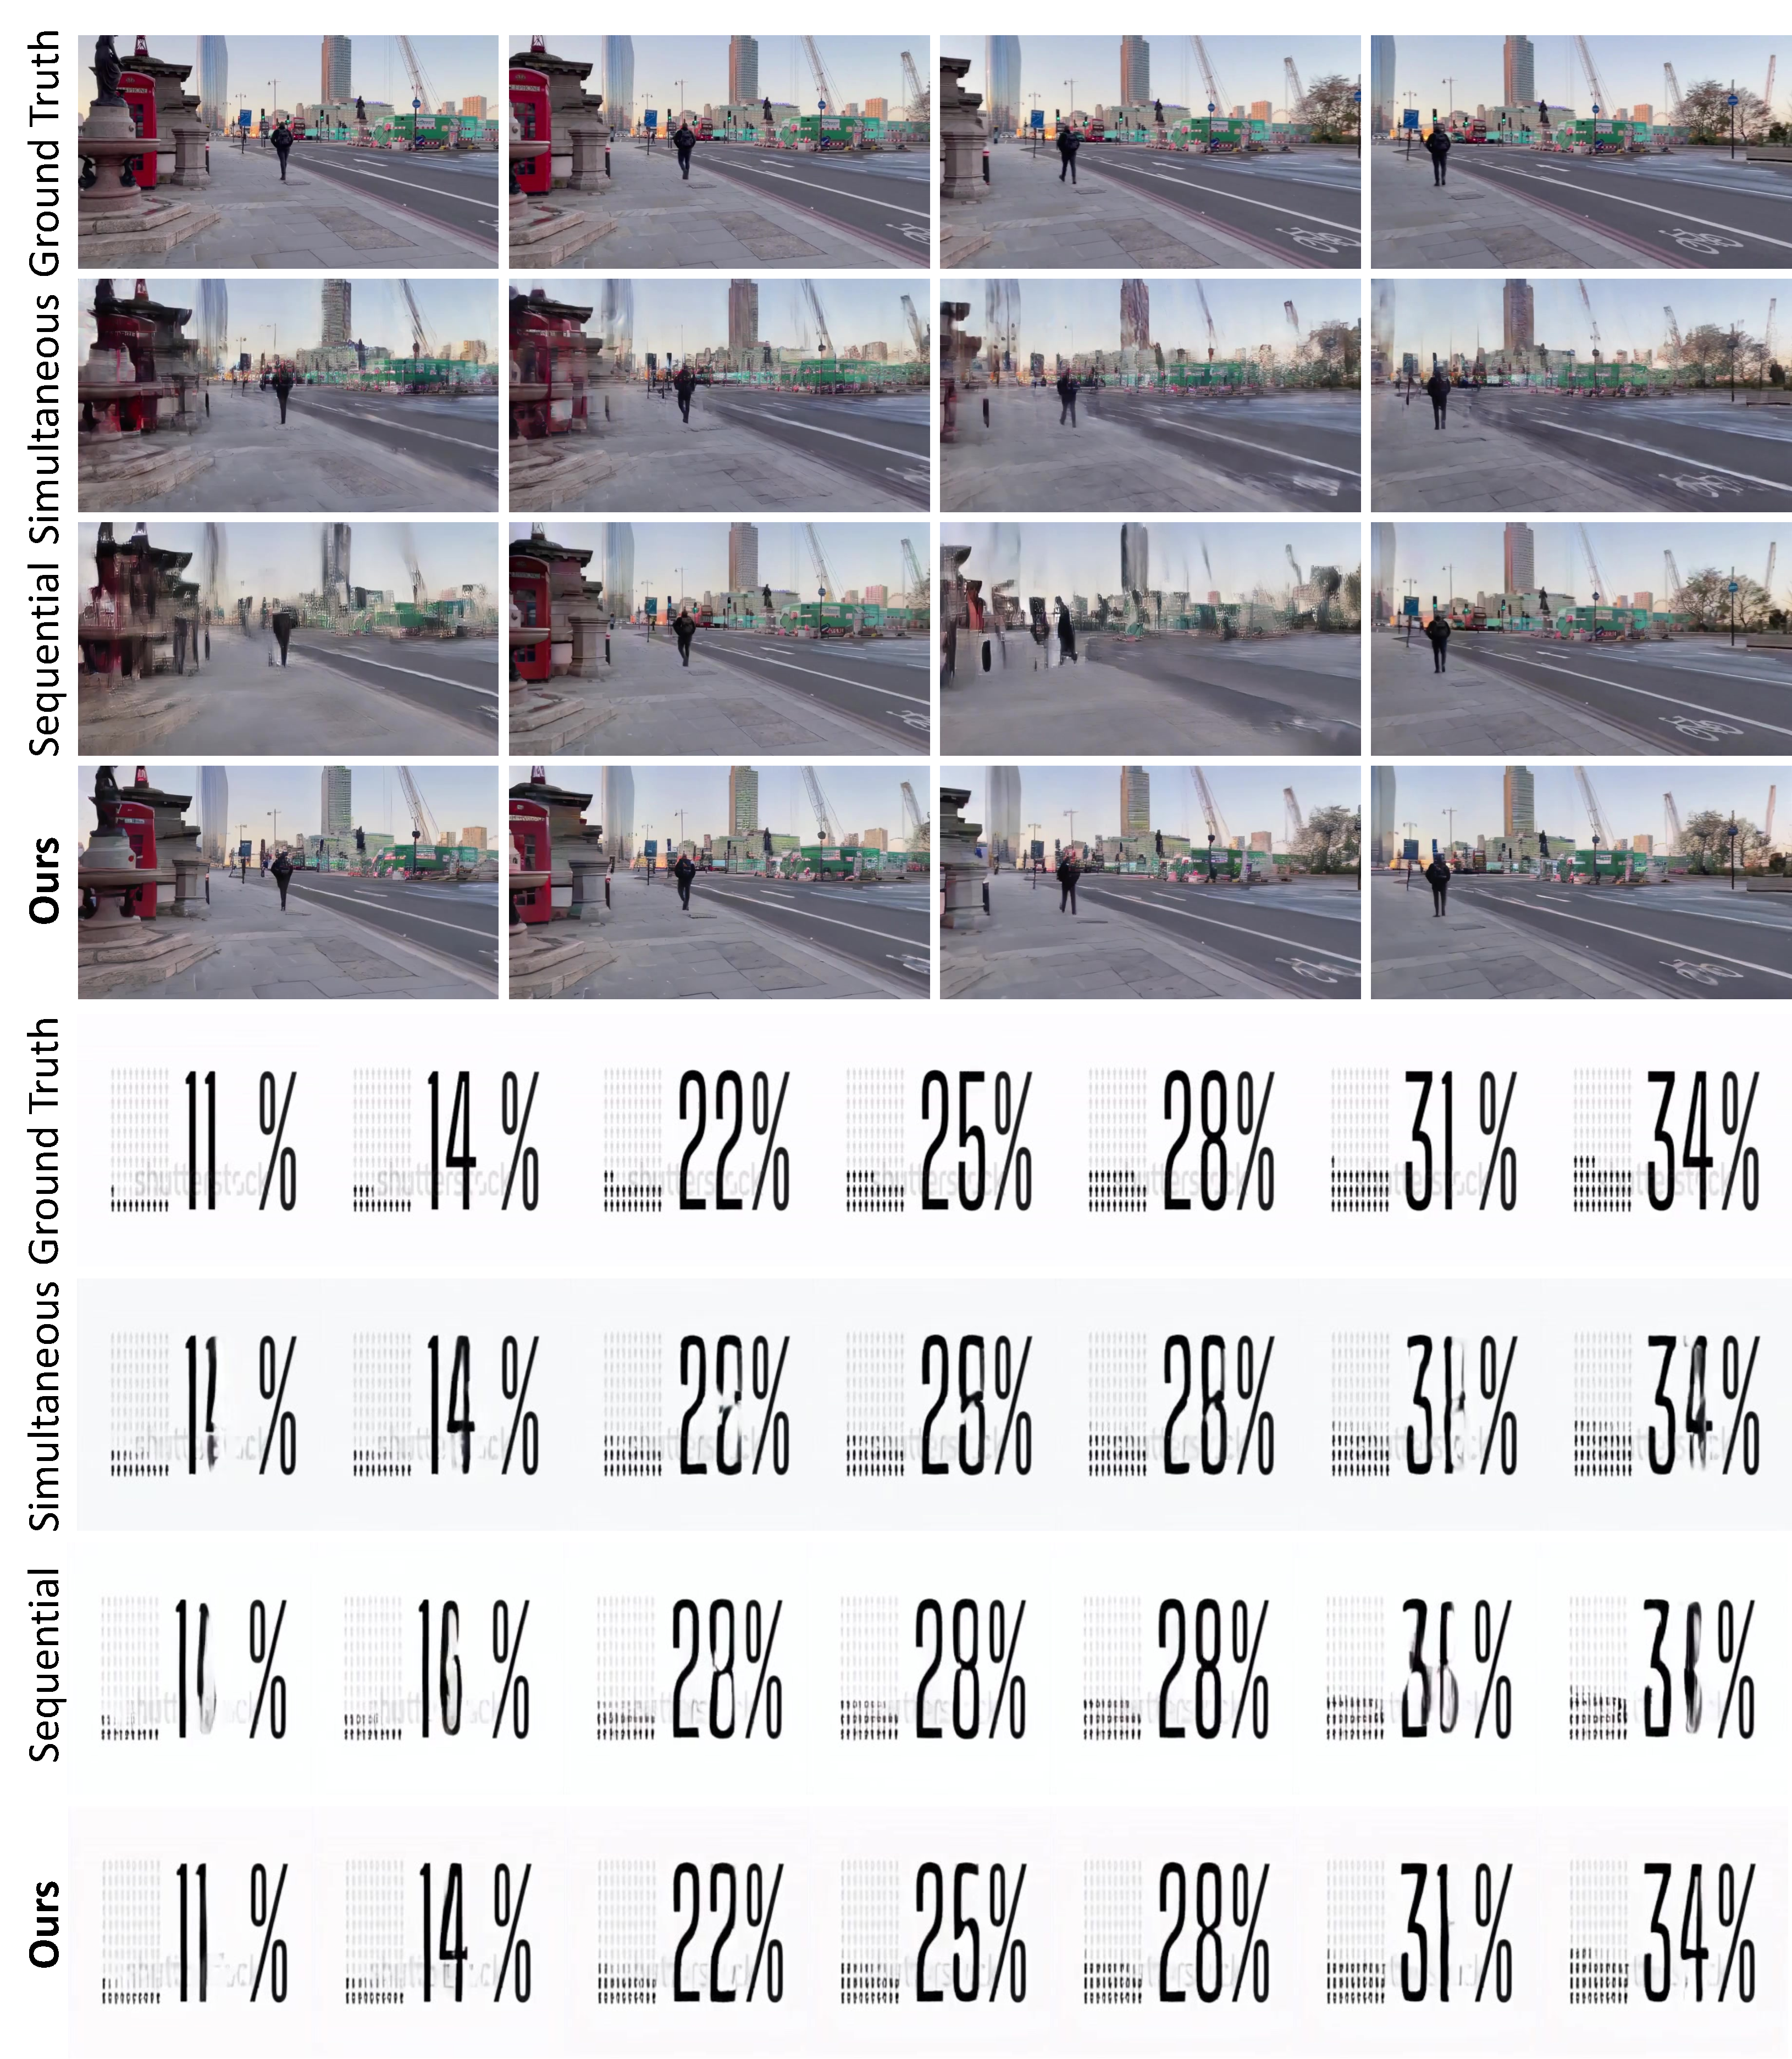
\includegraphics[width=0.8\textwidth]{images/aba-arch.pdf}
\caption{Comparisons among simultaneous spatiotemporal modeling, sequential spatiotemporal modeling and our proposed solution. 
}
\label{fig:modeling}
\vspace{-3mm}
\end{figure*}



\subsection{Loss Functions}
We use the reconstruction loss, the KL divergence loss, and the video adversarial loss (3D GAN loss) to optimize our model. 
The reconstruction loss, $\mathcal{L}_{\text{recon}}$, ensures that the generated frames are perceptually and structurally similar to the input frames. It combines a pixel-wise error term with a perceptual loss, weighted by a hyperparameter.
The KL divergence loss, $\mathcal{L}_{\text{KL}}$, regularizes the latent space by encouraging it to conform to a prior distribution, ensuring smoothness and continuity in the learned latent representations. Given the hierarchical structure of our latent space, we only regularize the innermost latent $\mathbf{Z_2}$, with dimensions $\frac{T}{4} \times \frac{H}{8} \times \frac{W}{8}$, where $T$, $H$, and $W$ represent the temporal, height, and width dimensions, respectively. The 3D GAN loss, $\mathcal{L}_{\text{GAN}}$, is introduced to enhance the realism of the generated video sequences, leveraging a discriminator to distinguish between real and generated sequences.
The total loss function is expressed as:

\begin{equation}
    \mathcal{L}_{\text{total}} = \mathcal{L}_{\text{recon}} + \lambda_{\text{KL}} \mathcal{L}_{\text{KL}} + \lambda_{\text{GAN}} \mathcal{L}_{\text{GAN}}.
\end{equation}

